
\begin{multicols}{2}

    \subsection{Systèmes de coordonnées}
    
    \subsubsection*{Coordonnées cylindriques}


    \begin{center}
        \includegraphics[width=0.4\textwidth]{figures/cylindriques.png}
    \end{center}

    On représente un point $\vec{M}$ par les trois coordonnées $\rho$, $\varphi$ and $z$:
    \begin{align*}
        \vec{M} = (\rho, \varphi, z).
    \end{align*}
    Les vecteurs unitaires sont représentés en base cartésienne comme:
    \begin{align*}
        \vec{e_\rho} = \begin{pmatrix} 
            \cos \varphi \\
            \sin \varphi \\
            0
        \end{pmatrix}, & 
        \vec{e_\rho} = \begin{pmatrix} 
            - \sin \varphi \\
            \cos \varphi \\
            0
        \end{pmatrix}, & 
        \vec{e_\rho} = \begin{pmatrix} 
            0 \\
            0 \\
            1
        \end{pmatrix}.
    \end{align*}
    On pose les coordonnées d'un point (et leur dérivées) comme suit: 
    \begin{align*}
        \vec{r} = \rho \vec{e_\rho} + z \vec{e_z}, \\
        \vec{v} = \dot{\vec{r}} = \dot{\rho} \vec{e_\rho} + \rho \dot{\varphi} \vec{e_\varphi} + \dot{z} \vec{e_z}, \\
        \vec{a} = \dot{\vec{v}} = \ddot{\vec{r}}, \\
        \ddot{\vec{r}} = (\ddot{\rho} - \rho \dot{\phi}^2) \vec{e_\rho} + (\rho \ddot{\varphi} + 2 \dot{\rho} \dot{\varphi}) \vec{e_\varphi} + \ddot{z} \vec{e_z}.
    \end{align*}
    
    \subsubsection*{Coordonnées sphériques}

    \begin{center}
        \includegraphics[width=0.4\textwidth]{figures/spheriques.png}
    \end{center}
        

    On représente un point $\vec{M}$ par les trois coordonnées $r$, $\theta$ and $\varphi$:
    \begin{align*}
        \vec{M} = (r, \theta, \varphi).
    \end{align*}
    Les vecteurs unitaires sont représentés en base cartésienne comme:
    \begin{align*}
        \vec{e_r} = \begin{pmatrix} 
            \sin \theta \cos \varphi  \\
            \sin \theta \sin \varphi \\
            \cos \theta
        \end{pmatrix}, & 
        \vec{e_\theta} = \begin{pmatrix} 
            \cos \varphi \cos \varphi \\
            \cos \varphi \sin \varphi \\
            - \sin \theta
        \end{pmatrix}, \\
        \vec{e_\varphi} = \begin{pmatrix} 
            -\sin \varphi \\
            \cos \varphi \\
            0
        \end{pmatrix}.
    \end{align*}
    On pose les coordonnées d'un point (et leur dérivées) comme suit:
    \begin{align*}
        \vec{r} = r \vec{e_r}, \\
        \vec{v} = \dot{\vec{r}} = \dot{r} \vec{e_r} + r \dot{\theta} \vec{e_\theta} + \sin \theta \vec{e_\varphi}, \\
        \vec{a} = \dot{\vec{v}} = \ddot{\vec{r}}, \\
        \ddot{\vec{r}} = (\ddot{r} - r \dot{\theta}^2 - r \dot{\varphi}^2 \sin^2 \theta) \vec{e_r}  \\
        + (r \ddot{\theta} + 2 \dot{r} \dot{\theta} - r \dot{\varphi}^2 \sin \theta \cos \theta) \vec{e_\theta} \\
        + (r \ddot{\varphi} \sin \theta + 2 \dot{r} \dot{\varphi}\sin\theta + 2 r \dot{\varphi} \dot{\theta} \cos \theta) \vec{e_\varphi}.
    \end{align*}
    
    \subsection{Equations différentielles}
    
    En physique 1 on traite des équations différentielles linéaire du premier et du second ordre. Physique 1 n'est pas un cours de math (en tout cas pas un cours sur les equations différentielles), donc on se contente d'étudier des equations différentielles connues. \textbf{La résolution de ces équations revient à réécrire les équations du mouvement sous une forme dont on connait déjà la solution}. 
    
    \subsubsection*{Marche à suivre pour résoudre une équation différentielle}

    \begin{enumerate}
        \item Identifier quel type d'équation on a (1er ordre, 2ème ordre, amorti ou non)
        \item Réécrire l'équation sous la forme canonique (pour la lisibilité)
        \item Résoudre
        \begin{enumerate}
            \item trouver la solution particulière
            \item trouver la solution homogène
        \end{enumerate}
        \item Trouver les inconnues en fonction des conditions initiales
    \end{enumerate}
    
    % \subsubsection*{Equations différentielles du premier ordre}

    % \begin{tikzpicture}
    %     \begin{axis}[
    %         legend pos = south east,
    %         xmin = 0, xmax = 30,
    %         ymin = -2, ymax = 4.0,
    %         xtick distance = 3,
    %         ytick distance = 2,
    %         grid = both,
    %         minor tick num = 1,
    %         major grid style = {lightgray},
    %         minor grid style = {lightgray!25},
    %         width = 0.45\textwidth,
    %         height = 0.4\textwidth]
    %         \addplot[
    %             domain = 0:30,
    %             samples = 200,
    %             smooth,
    %             thick,
    %             black,
    %         ] {-3*exp(-0.5*x)+2};
    %         \addplot[
    %             domain = 0:30,
    %             samples = 200,
    %             smooth,
    %             thick,
    %             blue,
    %         ] {-3*exp(-0.5*x)};
    %         \addplot[
    %             domain = 0:30,
    %             samples = 200,
    %             smooth,
    %             thick,
    %             red,
    %         ] {2 };
    %         \legend{$x(t)$ ,$x_h(t)$ ,$x_\text{part}$}
    %     \end{axis}
    % \end{tikzpicture}

    % La forme canonique est la suivante.
    % \begin{align*}
    %     \dot{x}(t) +  ax(t) = c.
    % \end{align*}
    % Intuition de ce que l'équation représente : frottements fluides (l'objet soumis aux frottements freine proportionnellement à sa vitesse). Utilisé pour modéliser la \textit{chute libre}, la \textit{vitesse d'un bateau} etc.
    % \BlankLine
    % Pour trouver la \textbf{solution particulière} on pose $\dot{x} = 0$, et donc $x(t)$ constant. La solution particulière est une constante. L'intuition derrière la solution particulière est "\textit{quel est le comportement à l'équilibre ?}".
    % \begin{align*}
    %     \overbrace{\dot{x}_\text{part}(t)}^{=0} +  ax_\text{part} = c,\\
    %     \iff ax_\text{part} = c.\\
    % \end{align*}
    % La \textbf{solution particulière} vaut donc  : 
    % \[x_\text{part} = \frac{c}{a}.  \tag{1}\]
    % Pour trouver la \textbf{solution homogène} on pose $c = 0$. La solution homogène est une fonction. L'intuition derrière la solution homogène est "\textit{quelle est la dynamique du système autour de son équilibre ?}".
    % \begin{align*}
    %     \dot{x_h}(t) +  ax_\text{h}(t) = \overbrace{c}^{=0},\\
    %     \iff \frac{dx_h(t)}{dt} +  ax_\text{h}(t) = 0,\\
    %     \iff \frac{dx_h(t)}{dt} = -  ax_\text{h}(t). \tag{2}\\ 
    % \end{align*}
    % La fonction qui vérifie $(2)$ (et constitue la solution homogène) est la suivante:
    % \[ x_h(t) = A \cdot e^{-a(t-t_0)}. \tag{3} \]
    % On trouve la solution de l'équation en additionnant les solutions homogène et partielle $(1)$ et $(3)$:
    % \begin{align*}
    %     x(t) = x_h(t) + x_\text{part}, \\
    %     x(t) = A \cdot e^{-a(t-t_0)}  + \frac{c}{a}.
    % \end{align*}
    % Les constantes $A$ et $t_0$ sont dépendantes des conditions initiales et se calculent en posant:
    % \begin{align*}
    %     x(t=0) =  x_\text{init}, \\
    %     \dot{x}(t=0) =  v_\text{init}.
    % \end{align*}

    % \subsubsection*{Equations différentielles du deuxième ordre (non amorti)}

    % \begin{tikzpicture}
    %     \begin{axis}[
    %         legend pos = south east,
    %         xmin = 0, xmax = 30,
    %         ymin = -2, ymax = 4.0,
    %         xtick distance = 3,
    %         ytick distance = 2,
    %         grid = both,
    %         minor tick num = 1,
    %         major grid style = {lightgray},
    %         minor grid style = {lightgray!25},
    %         width = 0.45\textwidth,
    %         height = 0.4\textwidth]
    %         \addplot[
    %             domain = 0:30,
    %             samples = 200,
    %             smooth,
    %             thick,
    %             black,
    %         ] {cos(100*x) + 2 };
    %         \addplot[
    %             domain = 0:30,
    %             samples = 200,
    %             smooth,
    %             thick,
    %             blue,
    %         ] {cos(100*x)};
    %         \addplot[
    %             domain = 0:30,
    %             samples = 200,
    %             smooth,
    %             thick,
    %             red,
    %         ] {2 };
    %         \legend{$x(t)$ ,$x_h(t)$ ,$x_\text{part}$}
    %     \end{axis}
    % \end{tikzpicture}

    % La forme canonique est la suivante.
    % \begin{align*}
    %     \ddot{x}(t) +  \omega_0^2 x(t) = c.
    % \end{align*}
    % Intuition de ce que l'équation représente : oscillateurs harmoniques (l'objet est rappelé vers un équilibre sans frottement et oscille à l'infini). Utilisé pour modéliser les oscillations d'un \textit{pendule}, d'un \textit{ressort} etc.

    % \BlankLine
    % Pour trouver la \textbf{solution particulière} on pose $\ddot{x} = 0$, et donc $x(t)$ constant. La solution particulière est une constante. L'intuition derrière la solution particulière est "\textit{quel est le comportement à l'équilibre ?}".
    % \begin{align*}
    %     \overbrace{\ddot{x}_\text{part}(t)}^{=0} +  \omega_0^2 x_\text{part} = c,\\
    %     \iff \omega_0^2 x_\text{part} = c.\\
    % \end{align*}
    % La \textbf{solution particulière} vaut donc  : 
    % \[x_\text{part} = \frac{c}{\omega_0^2}.  \tag{1}\]
    % Pour trouver la \textbf{solution homogène} on pose $c = 0$. La solution homogène est une fonction. L'intuition derrière la solution homogène est "\textit{quelle est la dynamique du système autour de son équilibre ?}".
    % \begin{align*}
    %     \ddot{x_h}(t) +  \omega_0^2 x_\text{h}(t) = \overbrace{c}^{=0},\\
    %     \iff \frac{d^2x_h(t)}{dt^2} +  \omega_0^2 x_\text{h}(t) = 0,\\
    %     \iff \frac{d^2x_h(t)}{dt^2} = -  \omega_0^2 x_\text{h}(t). \tag{2}\\ 
    % \end{align*}
    % La fonction qui vérifie $(2)$ (et constitue la solution homogène) est la suivante:
    % \[ x_h(t) = A \cdot cos(\omega_0 t + \varphi ) \tag{3} \]
    % On trouve la solution de l'équation en additionnant les solutions homogène et partielle $(1)$ et $(3)$:
    % \begin{align*}
    %     x(t) = x_h(t) + x_\text{part}, \\
    %     x(t) =  x_h(t) = A \cdot cos(\omega_0 t + \varphi )  + \frac{c}{a}.
    % \end{align*}
    % Les constantes $A$ et $\varphi$ sont dépendantes des conditions initiales et se calculent en posant:
    % \begin{align*}
    %     x(t=0) =  x_\text{init}, \\
    %     \dot{x}(t=0) =  v_\text{init}.
    % \end{align*}

\end{multicols}
    \newpage
\subsection{Tableau des équations différentielles}
\begin{center}
    \begin{tabular}{ |c|c|c|c| } 
        \hline
        Nom de l'équation & Forme canonique & solution particulière & solution homogène \\
        \hline
        \hline
        \textit{Premier ordre} & $\dot{x}(t) +  ax(t) = c$ & $x_\text{part} = \frac{c}{a}$ & $x_h(t) = A \cdot e^{-a(t-t_0)}$\\
        \hline& \multicolumn{3}{|l|}{Solution complète : $x(t) = A \cdot e^{-a(t-t_0)}  + \frac{c}{a}$}  \\
        & \multicolumn{3}{|c|}{ 

            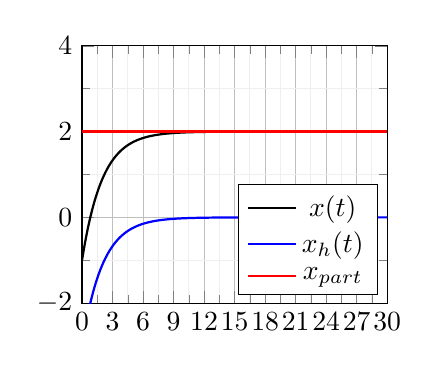
\begin{tikzpicture}
                \begin{axis}[
                    legend pos = south east,
                    xmin = 0, xmax = 30,
                    ymin = -2, ymax = 4.0,
                    xtick distance = 3,
                    ytick distance = 2,
                    grid = both,
                    minor tick num = 1,
                    major grid style = {lightgray},
                    minor grid style = {lightgray!25},
                    width = 0.45\textwidth,
                    height = 0.4\textwidth]
                    \addplot[
                        domain = 0:30,
                        samples = 200,
                        smooth,
                        thick,
                        black,
                    ] {-3*exp(-0.5*x)+2};
                    \addplot[
                        domain = 0:30,
                        samples = 200,
                        smooth,
                        thick,
                        blue,
                    ] {-3*exp(-0.5*x)};
                    \addplot[
                        domain = 0:30,
                        samples = 200,
                        smooth,
                        thick,
                        red,
                    ] {2 };
                    \legend{$x(t)$ ,$x_h(t)$ ,$x_\text{part}$}
                \end{axis}
            \end{tikzpicture}

         }  \\
        \hline
        \hline
        \textit{Deuxième ordre}& $ \ddot{x}(t) +  \omega_0^2 x(t) = c$ & $x_\text{part} = \frac{c}{\omega_0^2}$ & $x_h(t) = A \cdot cos(\omega_0 t + \varphi)$\\
        \hline \textit{oscillateur non amorti} & \multicolumn{3}{|l|}{Solution complète : $x(t) =  x_h(t) = A \cdot cos(\omega_0 t + \varphi )  + \frac{c}{a}$}  \\
        & \multicolumn{3}{|c|}{ 

            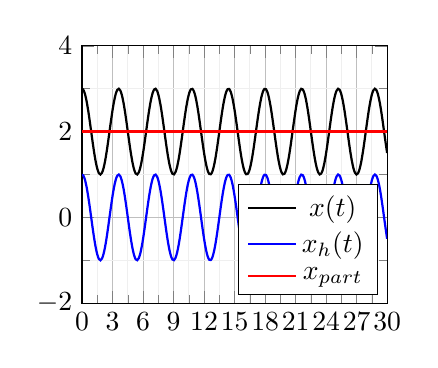
\begin{tikzpicture}
                \begin{axis}[
                    legend pos = south east,
                    xmin = 0, xmax = 30,
                    ymin = -2, ymax = 4.0,
                    xtick distance = 3,
                    ytick distance = 2,
                    grid = both,
                    minor tick num = 1,
                    major grid style = {lightgray},
                    minor grid style = {lightgray!25},
                    width = 0.45\textwidth,
                    height = 0.4\textwidth]
                    \addplot[
                        domain = 0:30,
                        samples = 200,
                        smooth,
                        thick,
                        black,
                    ] {cos(100*x) + 2 };
                    \addplot[
                        domain = 0:30,
                        samples = 200,
                        smooth,
                        thick,
                        blue,
                    ] {cos(100*x)};
                    \addplot[
                        domain = 0:30,
                        samples = 200,
                        smooth,
                        thick,
                        red,
                    ] {2 };
                    \legend{$x(t)$ ,$x_h(t)$ ,$x_\text{part}$}
                \end{axis}
            \end{tikzpicture}
        

         }  \\
        & \multicolumn{3}{|l|}{ Note : la solution homogène peut être réécrite $x(t) =  x_h(t) = A \cdot sin(\omega_0 t + \varphi )$  } \\
        & \multicolumn{3}{|l|}{ ou encore $x(t) =  x_h(t) = A \cdot sin(\omega_0 t) + B \cdot sin(\omega_0 t)$.} \\
        & \multicolumn{3}{|l|}{(En choisissant correctement les constantes).} \\
        \hline
        \hline
        \textit{Deuxième ordre}& $ a\ddot{x}(t) + b \dot{x}(t) + c x(t) = d$ & $x_\text{part} = \frac{d}{c}$ & $x_h(t)$ : plusieurs cas\\
        \hline \textit{oscillateur amorti} & \multicolumn{3}{|l|}{
            
        
            Coefficient d'amortissement: $\lambda = \frac{b}{2a}$, pulsation propre: $\frac{c}{a} =  \omega_0^2$

        }  \\
        & \multicolumn{3}{|l|}{
            1. $\lambda < \omega_0$ $\Rightarrow$ amortissement faible : $x_h(t) = Ae^{-\lambda t} cos(\omega t + \varphi)$, avec $\omega = \sqrt{\omega_0^2 - \lambda^2}$
        }  \\
        & \multicolumn{3}{|l|}{
            2. $\lambda > \omega_0$ $\Rightarrow$ amortissement fort : $x_h(t) = e^{-\lambda t} \left(C_1 e^{\omega t}+ C_2 e^{\omega t}\right)$, avec $\omega = \sqrt{\lambda^2 - \omega_0^2}$
        }  \\
        & \multicolumn{3}{|l|}{
            3. $\lambda = \omega_0$ $\Rightarrow$ amortissement critique : $x_h(t) = e^{-\lambda t} \left(C_1 + C_2 t\right)$
        }  \\
        & \multicolumn{3}{|c|}{ 

            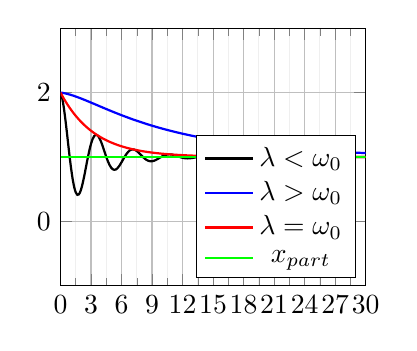
\begin{tikzpicture}
                \begin{axis}[
                    legend pos = south east,
                    xmin = 0, xmax = 30,
                    ymin = -1, ymax = 3.0,
                    xtick distance = 3,
                    ytick distance = 2,
                    grid = both,
                    minor tick num = 1,
                    major grid style = {lightgray},
                    minor grid style = {lightgray!25},
                    width = 0.45\textwidth,
                    height = 0.4\textwidth]
                    \addplot[
                        domain = 0:30,
                        samples = 200,
                        smooth,
                        thick,
                        black,
                    ] {exp(-0.3*x)*cos(100*x) + 1 };
                    \addplot[
                        domain = 0:30,
                        samples = 200,
                        smooth,
                        thick,
                        blue,
                    ]  {exp(-0.3*x) * (1.2*exp(0.2*x) -0.2*exp(-0.2*x) ) + 1 };
                    \addplot[
                        domain = 0:30,
                        samples = 200,
                        smooth,
                        thick,
                        red,
                    ] {exp(-0.3*x) * (1) + 1 };
                    \addplot[
                        domain = 0:30,
                        samples = 200,
                        smooth,
                        thick,
                        green,
                    ] {1 };
                    \legend{$\lambda < \omega_0$ ,$\lambda > \omega_0$ ,$\lambda = \omega_0$,$x_\text{part}$}
                \end{axis}
            \end{tikzpicture}
        

         }  \\
         & \multicolumn{3}{|l|}{
            La solution est toujours donnée par $x(t) = x_h(t) + x_\text{part}$.
        }  \\
        \hline
    \end{tabular}
\end{center}